\comment{-------Text from Noah's presentation to be included in this section----------}
I will now explain in a short and hopefully not too technical way how our e-voting protocol actually works. A company that wants to be part of our rating applies and sends their unverified data via smart contract to the blockchain. They also send bEquality the email addresses of all employees which we store in a secure and private database. We then send links to a chosen percentage of employees with which they can register a blockchain account and their new Ethereum address is automatically sent to our database. We load a small amount of Ethereum onto their account so that they can pay for one transaction. bEquality then creates a survey-contract on the blockchain and sends the link via an app to all employees so that they can fill in their answers directly onto the blockchain. After all the survey have been filled out, the data on the blockchain is analysed by our system and published on our website. Because the data is on the blockchain, everyone can verify the integrity of our analysis. Yet there are still challenges ahead of us, for example the possible storing of the Ethereum addresses on the blockchain instead of a private database for further transparency.
\comment{----------------------------------END TEXT------------------------------------------------------------}


-introduction to this part

\begin{figure}[H]
	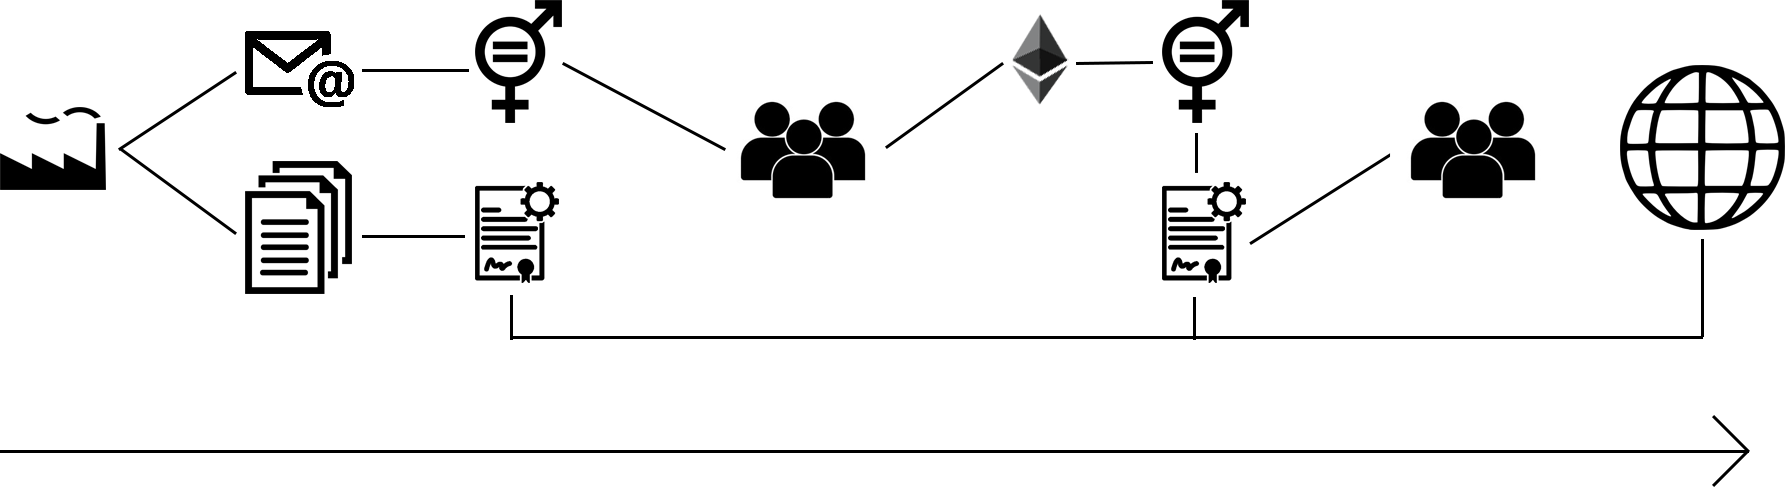
\includegraphics[width=0.9\textwidth]{Bilder/Survey_Protocol_preview_2}
	\caption{technical flow representation of the data capture and storage process}
	\label{technical_flow_representation}
\end{figure}
\comment{-------- insert picture of technical flow by Noah Berner}

\paragraph*{Survey for Employer}
-based on existing frameworks such as Bloomberg, Equileap\\
capturing data with app or web
-delivers e-mail addresses from employees\\
--addresses stored on private database\\
-survey stored on IPFS\\
-explain interaction with web/App\\


\paragraph*{Survey for Employees}

-are there existing questions for gender specific questions or not? Do we have to come up with questions which are applicable for men and/or women\\
-questions chosen possibly in a random manner.\\
-only percentage of employees (explain why only a percentage, mention pro's and con's)\\

capturing data with app or web\\
-explain,that process automated in the background\\
-what does the employee has to do\\
-what is done behind the scenes\\
	
storing data: blockchain, IPFS, (some on server)\\
-how is privacy of data secured\\
-explain process, what does this mean for different data\\
--sensibele data -- server\\
--insensible data -- ipfs\\
--non-fakeable -- blockchain\\
-explain cost aspect of storing stuff on blockchain or on IPFS (storing on blockchain costly)\\


how can anonymity/privacy be ensured\\
-because data on blockchain, IPFS, it is visible for everybody, but boss should not be able to track the results of employees (how do we solve that)\\

state technical problems

...


